\documentclass[12pt]{article}
\usepackage[margin=2.54cm]{geometry}
\usepackage[colorlinks,urlcolor=blue]{hyperref}
\usepackage{graphicx}


\title{CS 4480: PA1 Final Report}
\author{Jesus Zarate}
\date{February 13, 2017}

\begin{document}

\maketitle

The way I designed this was to have a socket listening for a connection. Once it received a connetion and the handshake
was successful then a new thread would start in order to listen for requests. I went with this approach because I didn't
want to deploy a new thread, and waste resources if the handshake wasn't successful. Once we start communicating the server
 will recognize when the user wants to execute a GET request and only a GET request. This server is able to take a relative
 URL as well as an absolute URL. After the URL has been specified the program will keep on listening for the headers, and
 once the user is done entering they can press enter once more to execute the command. A decision I made for my server was
 to close the connection once a request had been made. This made it easy to know if the request was successful or it was not.
 If the user wants to make another request they need to fire another socket.\\

 If the behaviour above conflicts with TA grading please let me know, and I can easily fix this in order to make the
 gradind easier, or if it's just not the behaviour you were looking for.\\

The way I tested this proxy was first to test it on other websites like the 'real simple' site, and other websites
like Google in order to check that the output was still good (the hash of the content). Then I created a simple
HTTP server with a known piece of malware. I checked the hash of that malware through team cymru and indeed they say it
was malware, then when I tried making a get request to my server with the URL pointing to the Malware it gives me back
a 200 response, and a warning saying that what I'm trying to access might contain Malware. Then I did the same, but with
a pdf file, and the response is a 200 response with the pdf.\\\\



Using the proxy making a request to http://www.cs.utah.edu/~kobus/simple.html we get a 200 response

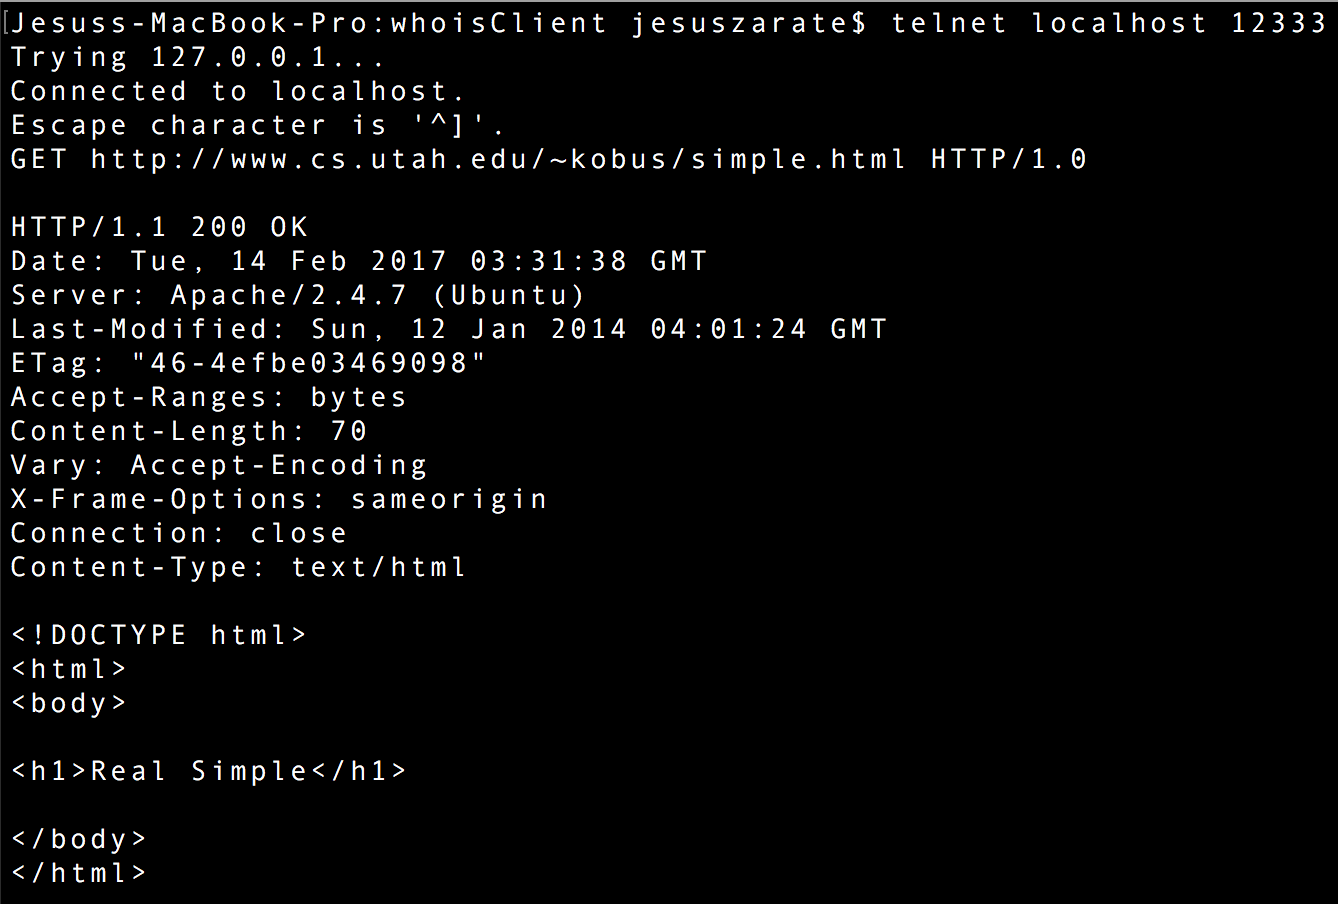
\includegraphics[width=.6\linewidth]{img/real_simple.png}


\\\\Now using the proxy making arequest to a local http server that contains a piece of malware \\


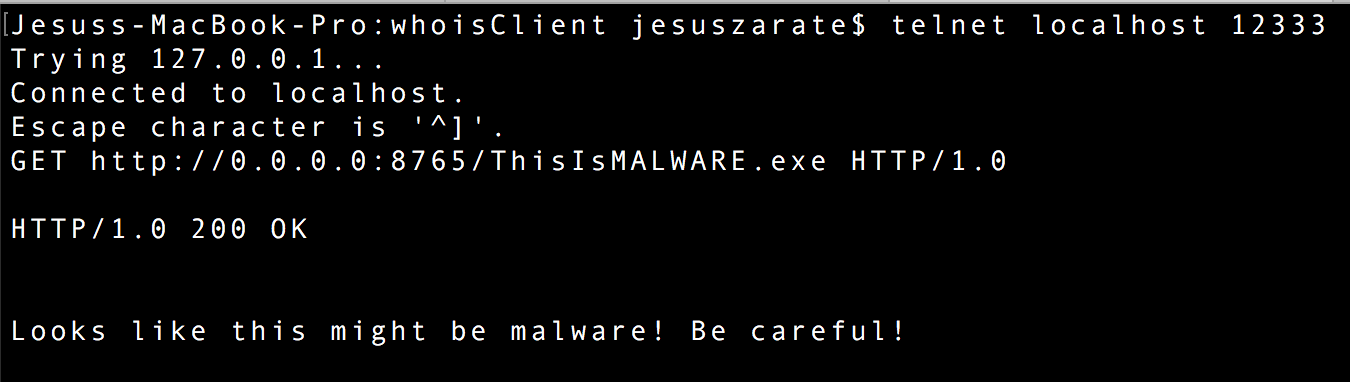
\includegraphics[width=.6\linewidth]{img/malware.png}



\end{document}
